\documentclass[12pt, letterpaper]{report}
\usepackage[margin=1in, headheight=41.68335pt, top=71.68335pt]{geometry}
\usepackage{amsmath}
\usepackage{amssymb}
\usepackage{fancyhdr}
\usepackage{pgfplots}
\usepackage{graphicx}
\pgfplotsset{compat=1.16}
\usepackage{hyperref} % Add this package for hyperlinks

\author{Gabriel Choong Ge Liang}
\title{Analysis of Sorting Algorithms}

\pagestyle{fancy}
\fancyhf{}
\renewcommand{\headrulewidth}{0pt}
\fancyhead[R]{%
    \begin{tabular}[b]{@{}r@{}}
    Gabriel Choong Ge Liang \\
    Assignment
    \end{tabular}%
}
\fancyfoot[R]{Page \thepage}

\begin{document}

\maketitle

\section*{1.1 Array Size}
Comparing each sorting algorithm with different array sizes.

\begin{figure}[htbp]
    \centering
    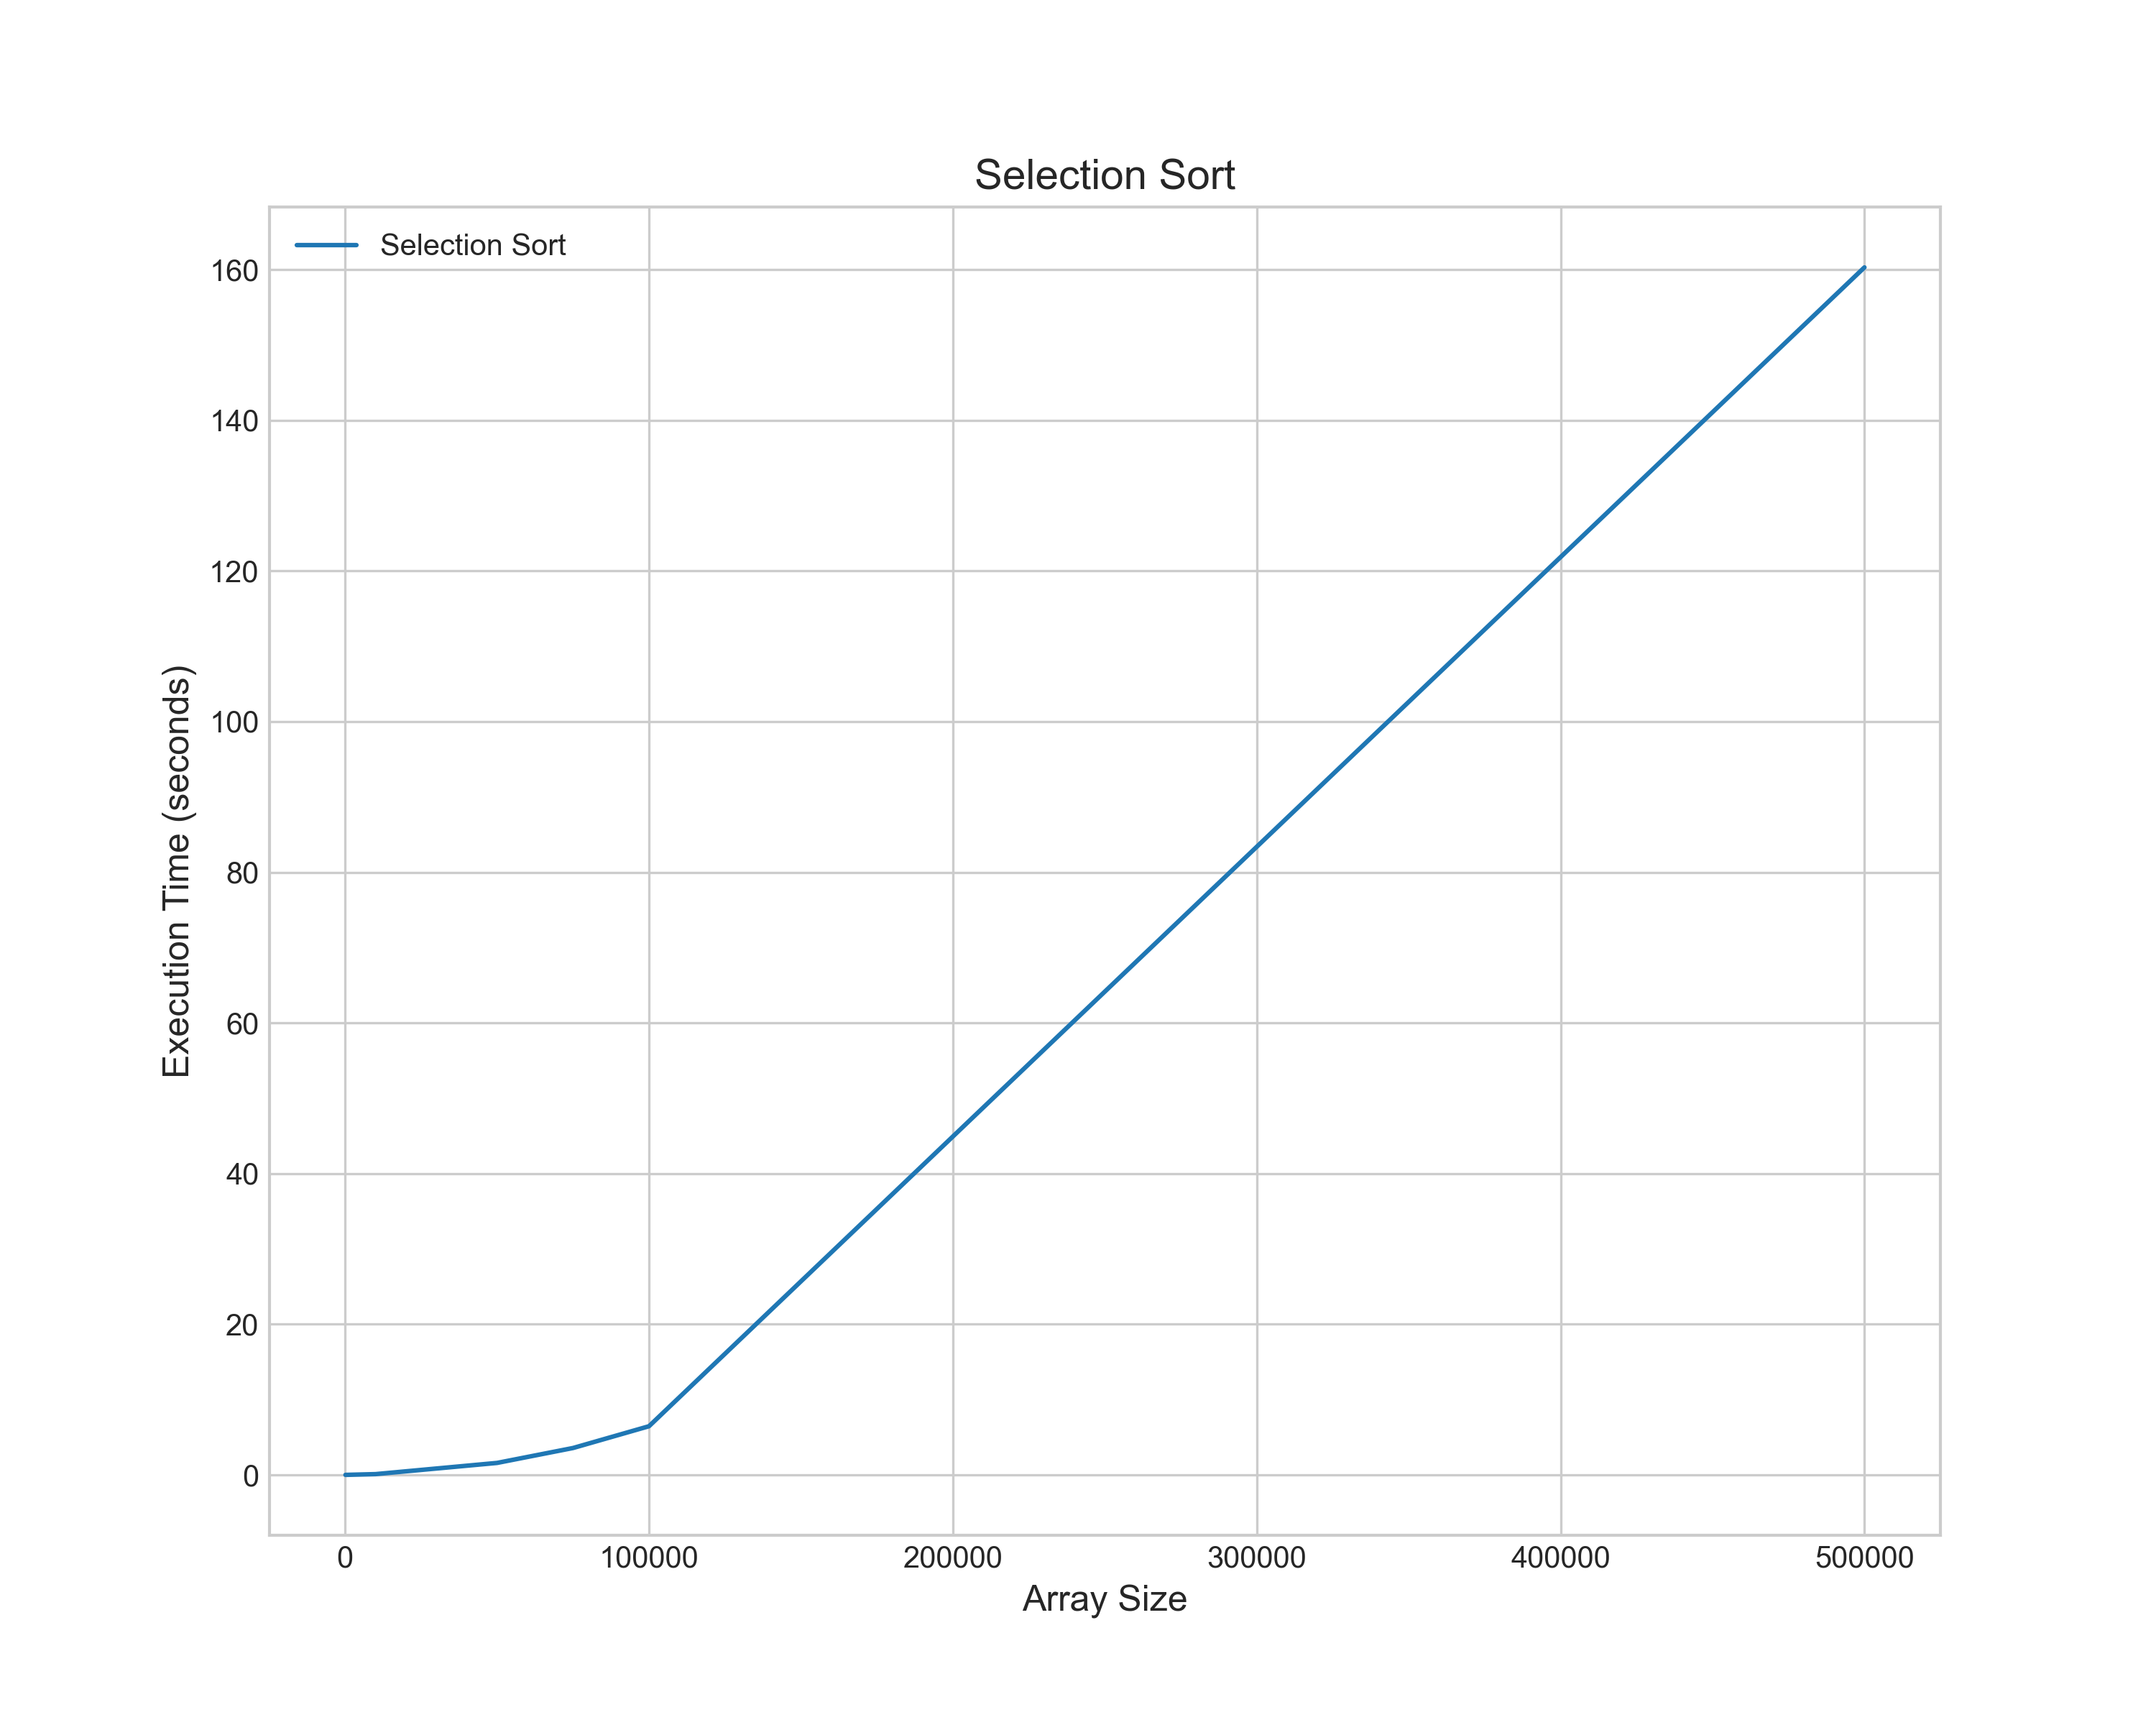
\includegraphics[width=0.5\textwidth]{"../img/a_selection_sort.png"}
    \caption{Comparison of Selection Sort with different array sizes.}
    \label{fig:image1}
\end{figure}

\begin{figure}[htbp]
    \centering
    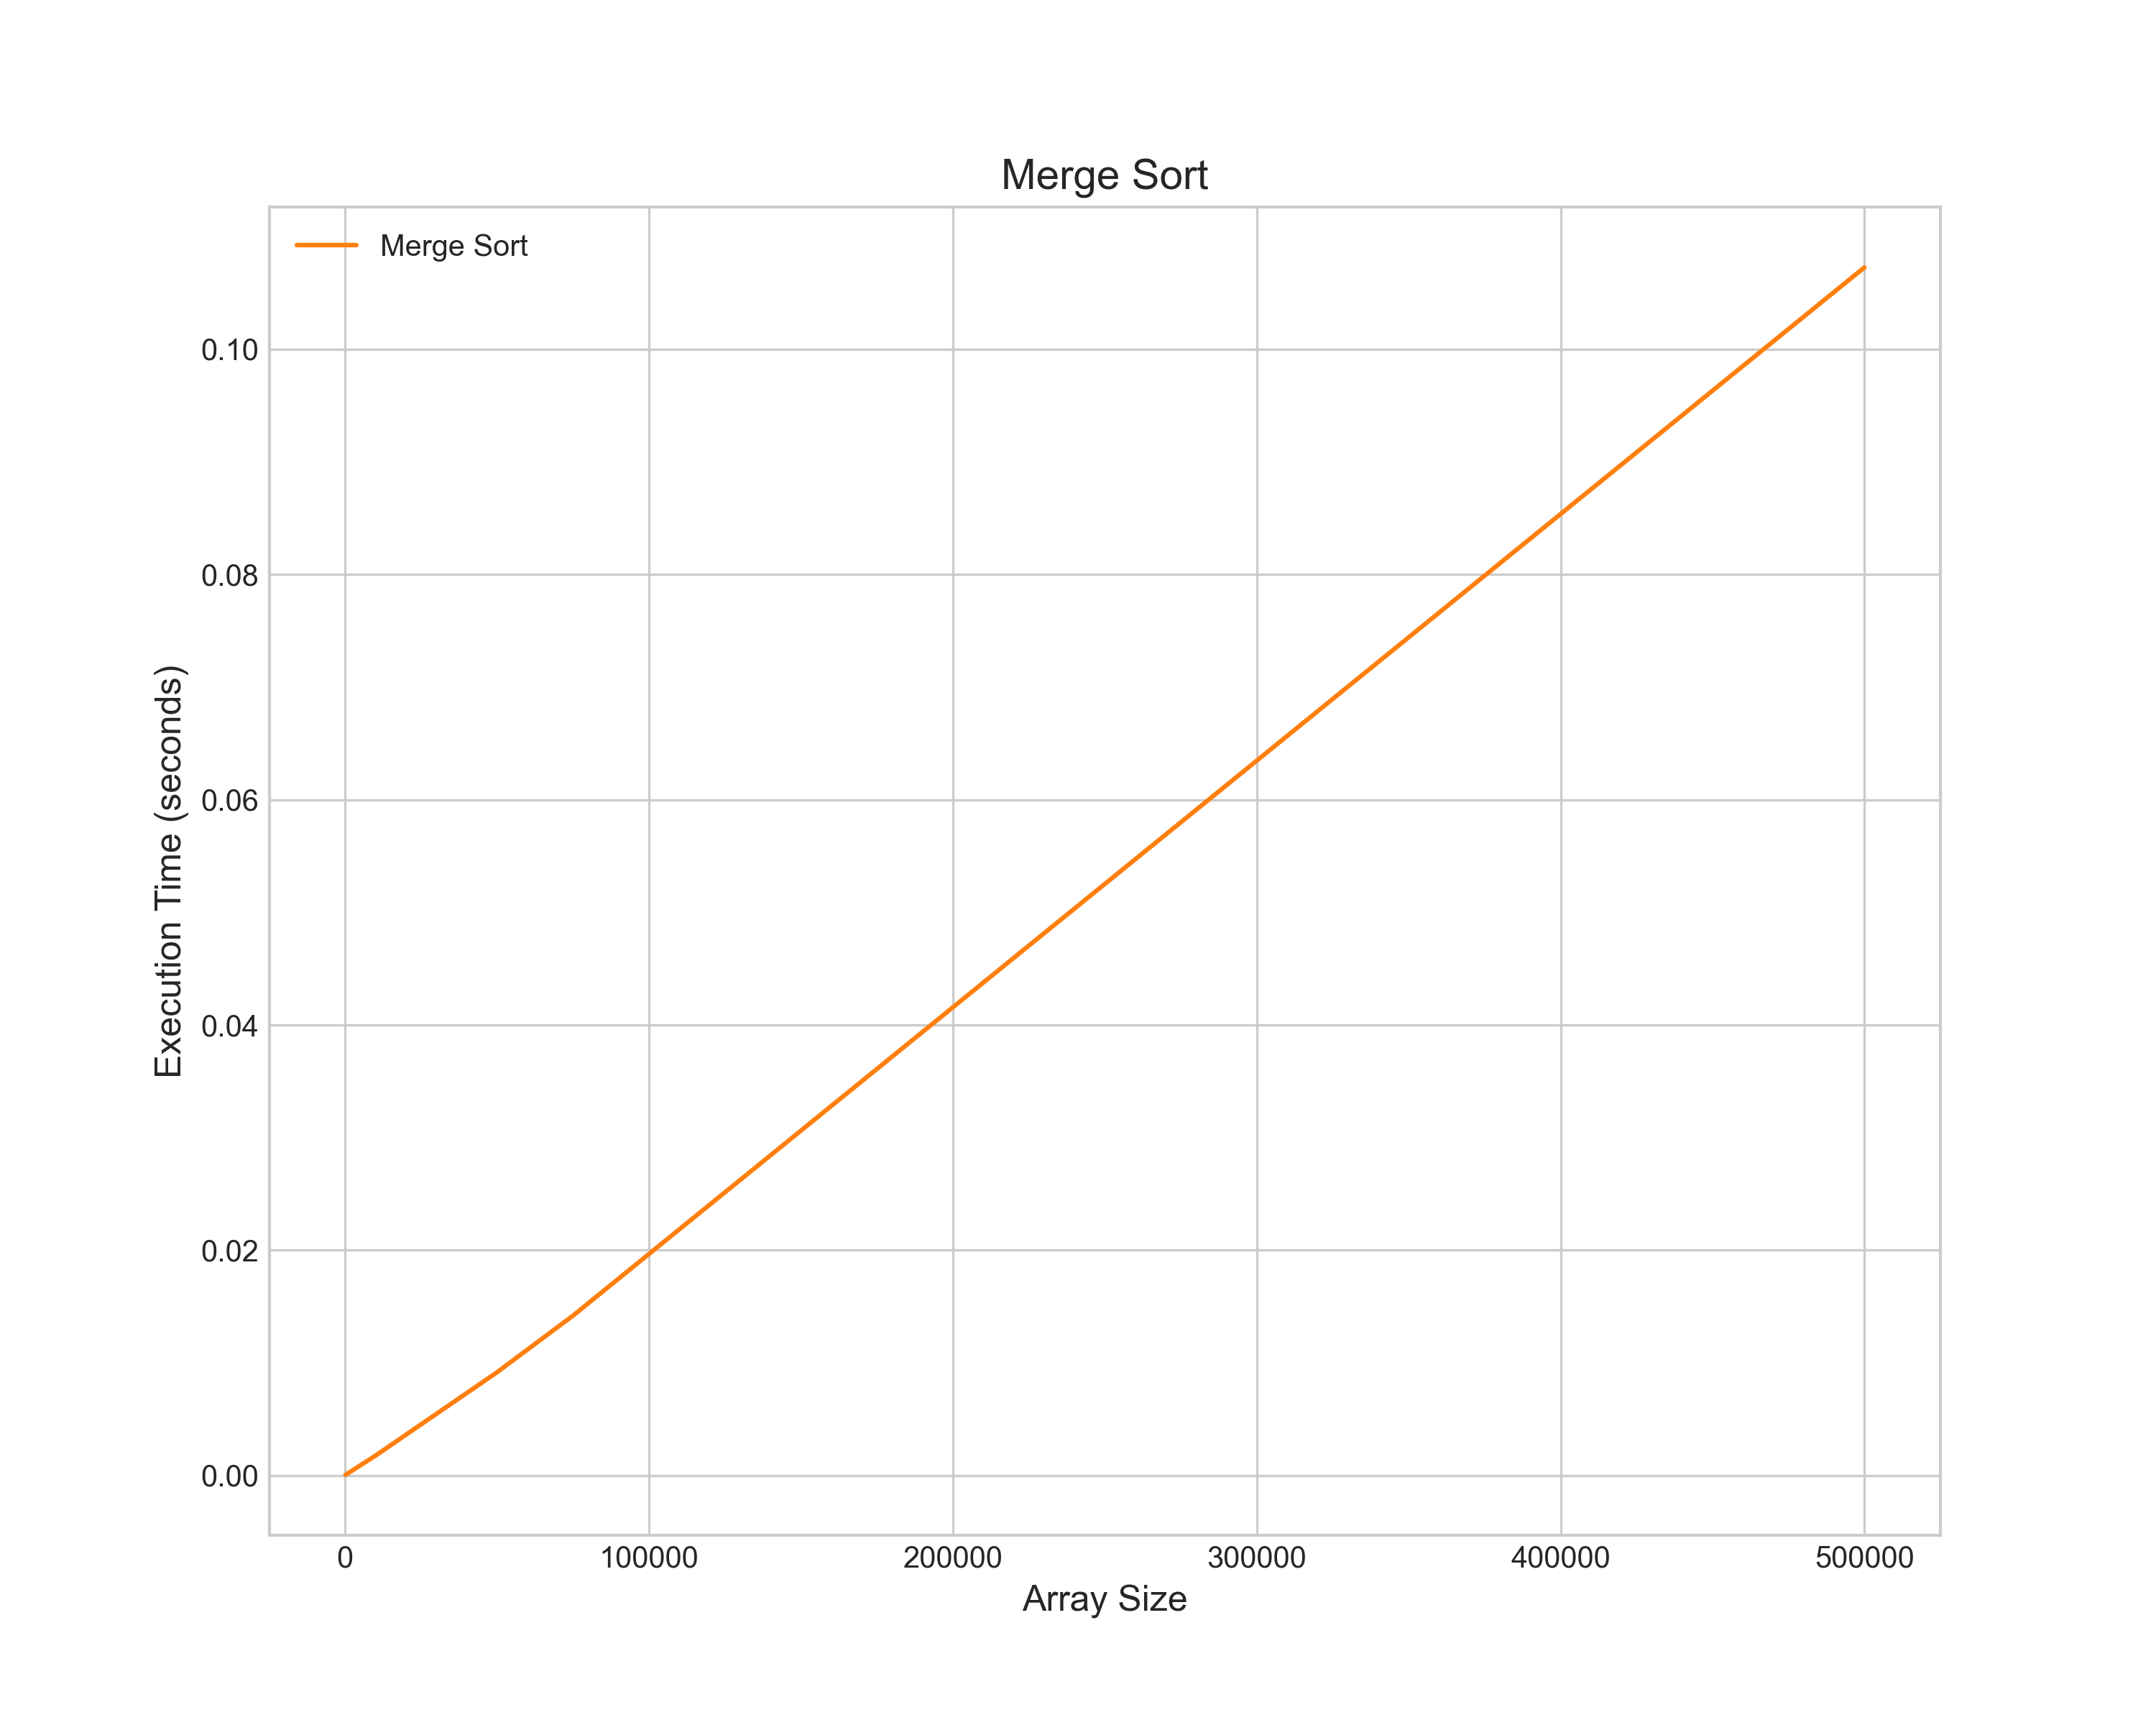
\includegraphics[width=0.5\textwidth]{"../img/a_merge_sort.png"}
    \caption{Comparison of Merge Sort with different array sizes.}
    \label{fig:image2}
\end{figure}

\begin{figure}[htbp]
    \centering
    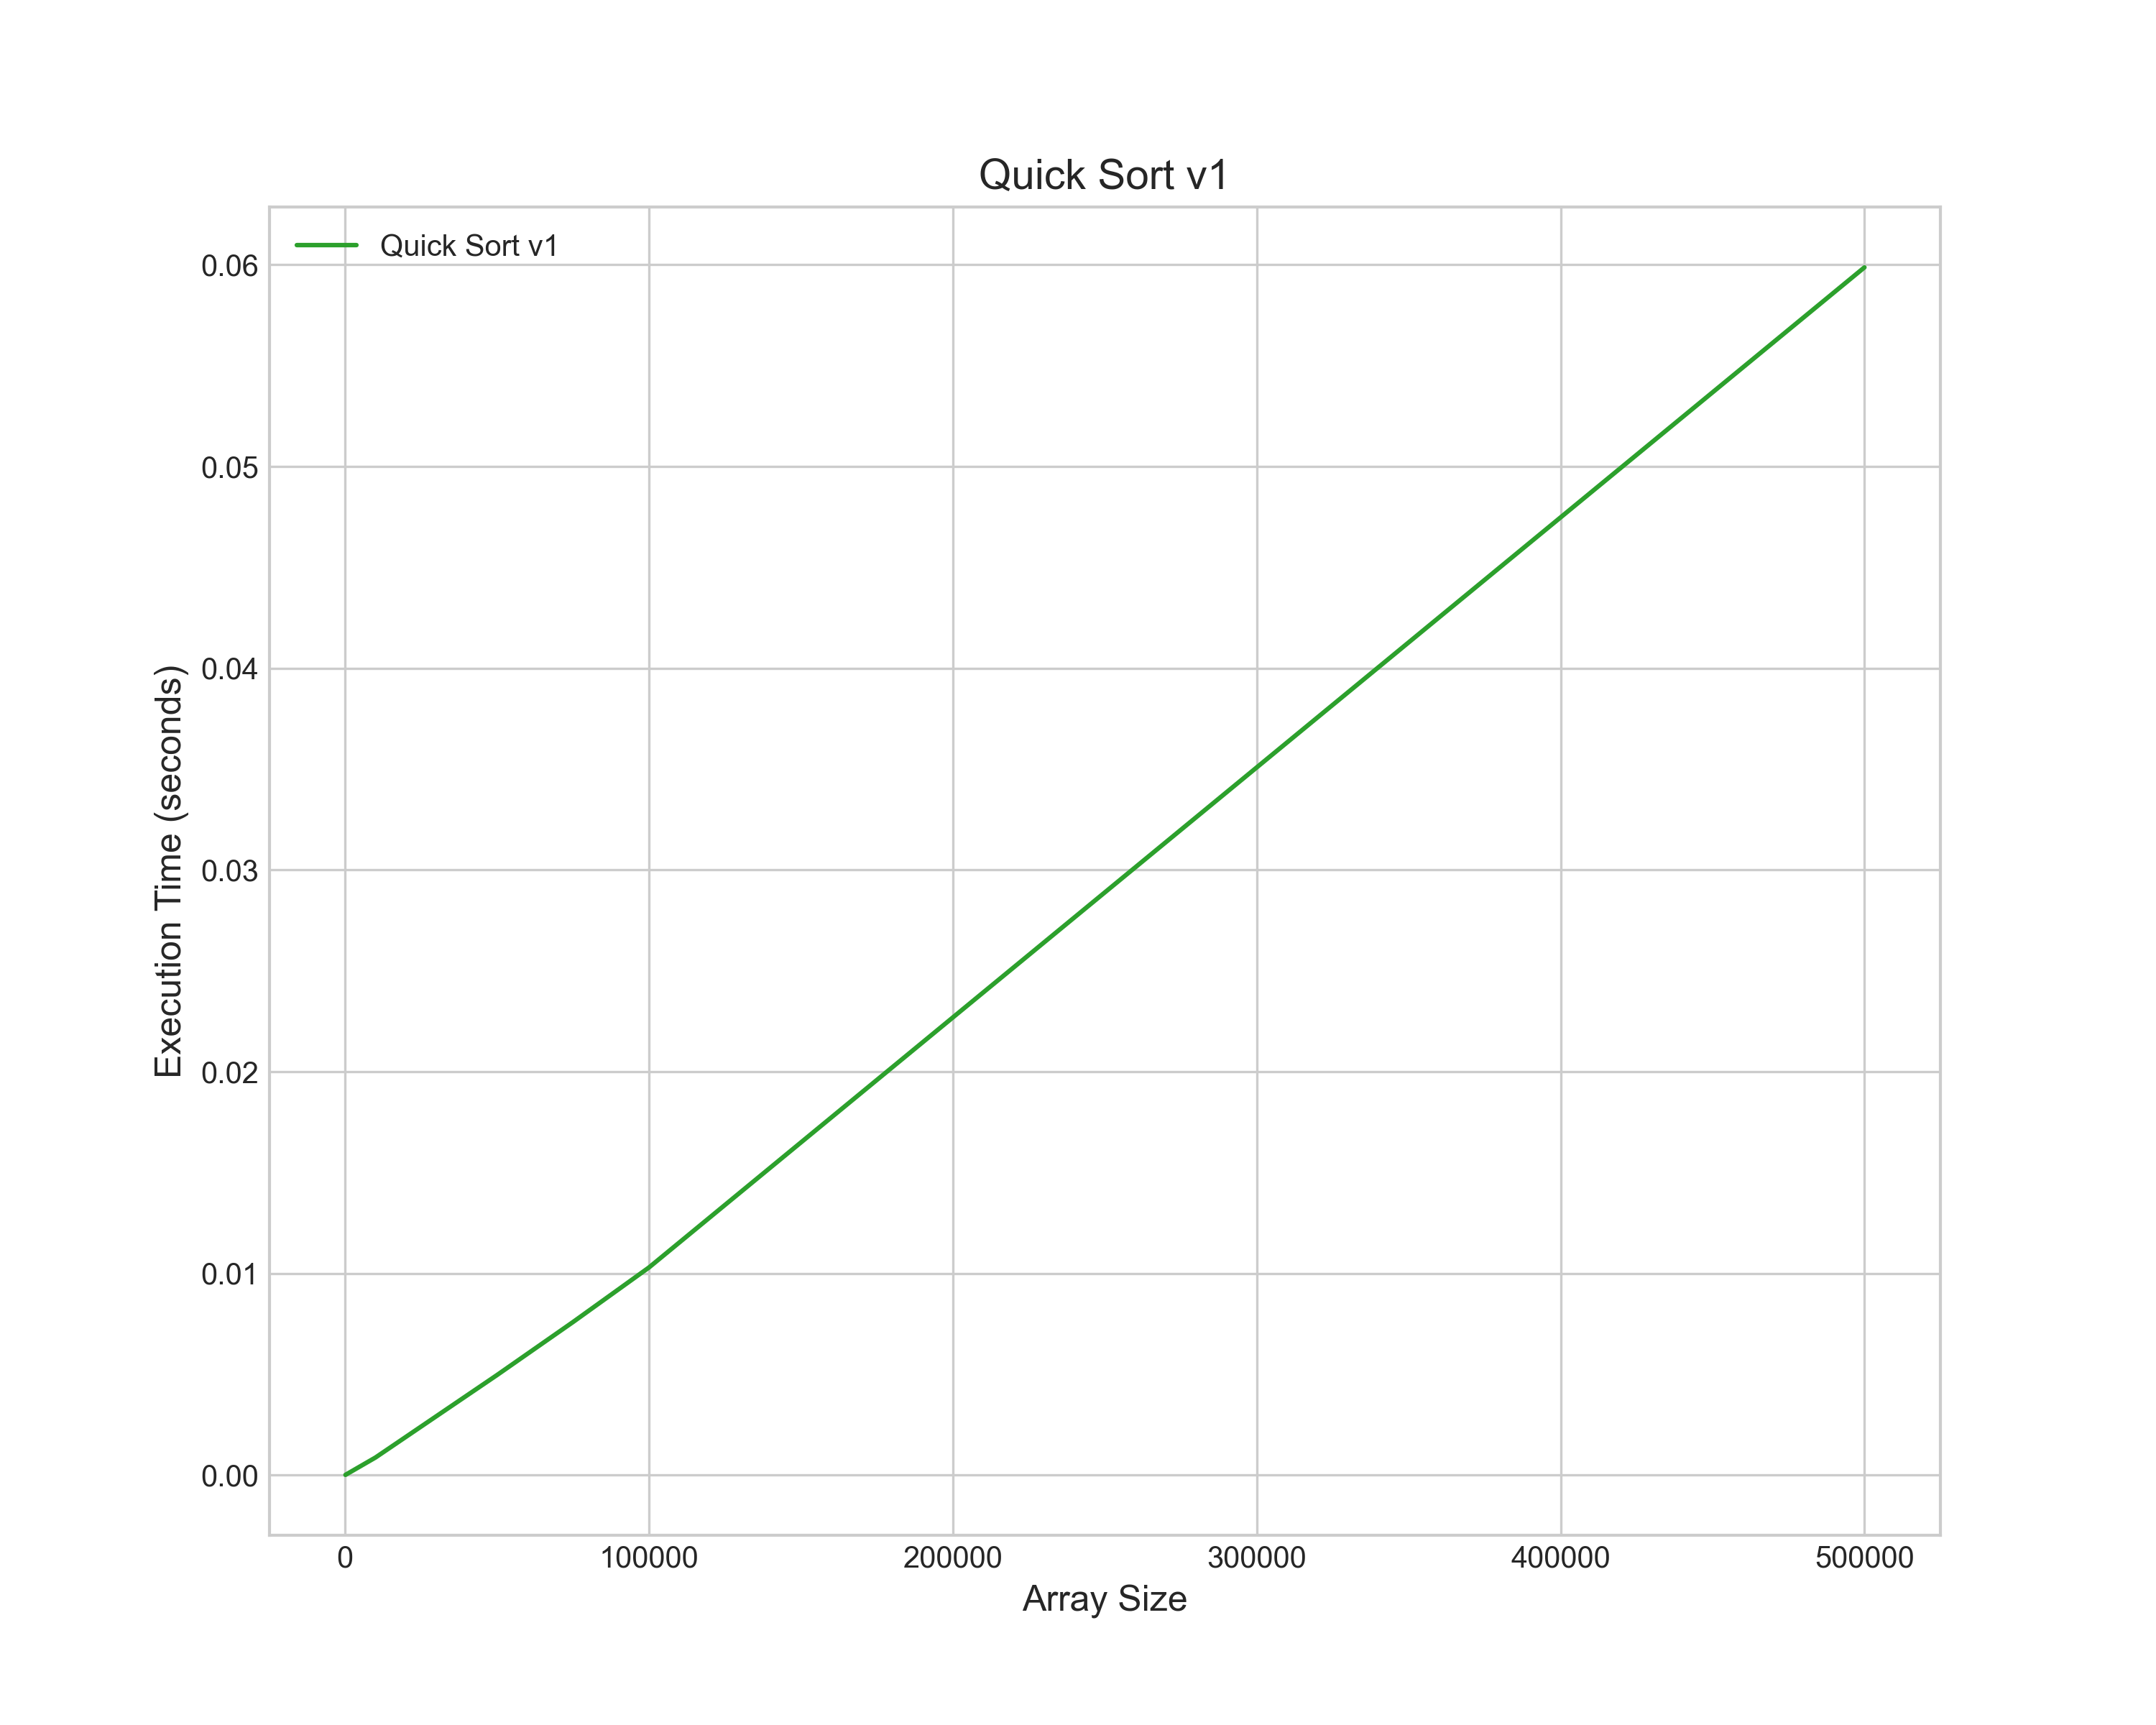
\includegraphics[width=0.5\textwidth]{"../img/a_quick_sort_v1.png"}
    \caption{Comparison of Quick Sort V1 with different array sizes.}
    \label{fig:image3}
\end{figure}

\begin{figure}[htbp]
    \centering
    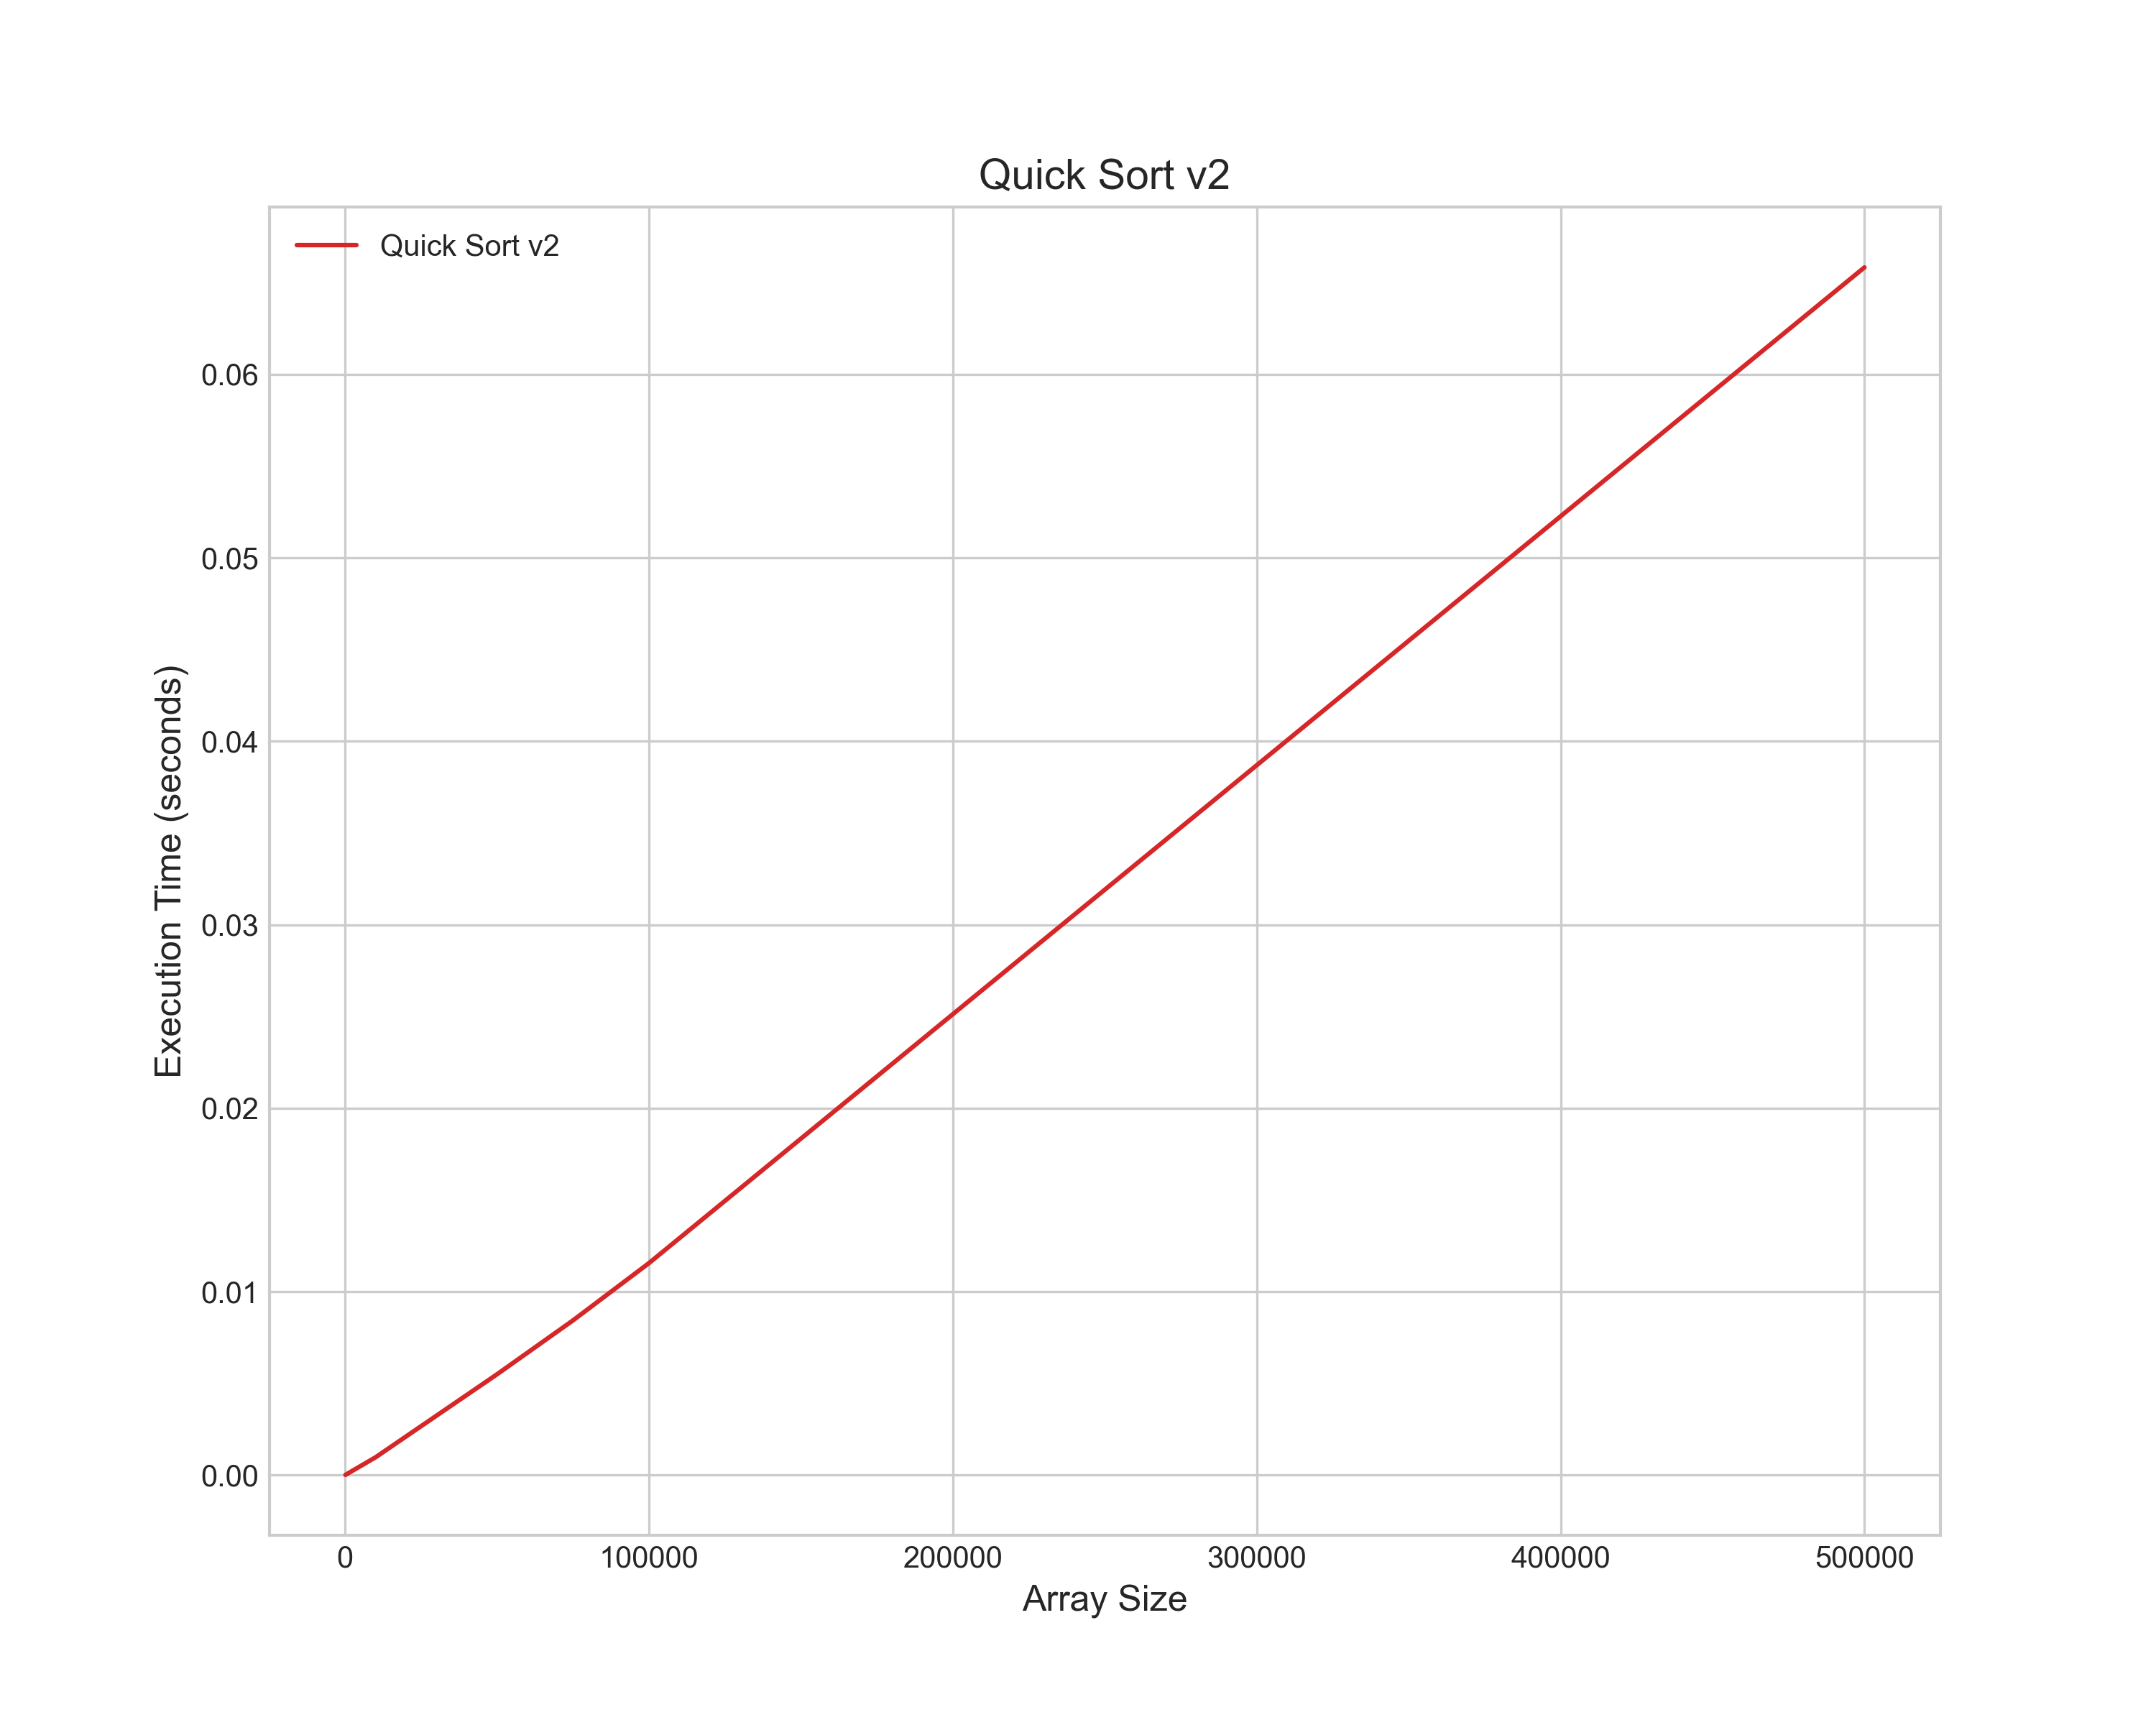
\includegraphics[width=0.5\textwidth]{"../img/a_quick_sort_v2.png"}
    \caption{Comparison of Selection Sort V2 with different array sizes.}
    \label{fig:image4}
\end{figure}

\clearpage

The graphs above compare the efficiency of sorting algorithms when the input array size varies. In Figure \ref{fig:image1}, the graph shows the quadratic function $x^2$. This is expected since Selection Sort has a time complexity of $O(n^2)$.

\par\medskip

Figure \ref{fig:image2} shows a curve that is close to a straight line. This is because Merge Sort has a time complexity of $O(n \log n)$. For large \(n\), Merge Sort is more efficient than Selection Sort.

\par\medskip

In Figure \ref{fig:image3} and Figure \ref{fig:image4}, we compare two versions of Quick Sort algorithms, differing only in the pivot selection. The graph shows that the pivot selection slightly affects the efficiency of the algorithm. Theoretically, the second version should be more efficient than the first version. However, the graph shows that the first version is more efficient than the second version. This is because the second version has a higher constant factor due to the pivot swap with the last element of the array, while the first version does not require such a swap. Thus, the first version of Quick Sort is more efficient than the second version. Other factors, such as the random number generator used to generate the array, can also contribute to this difference in efficiency.

\clearpage

\section*{1.2 Algorithm}
Comparing sorting algorithms on arrays with the same size.

\begin{figure}[htbp]
    \centering
    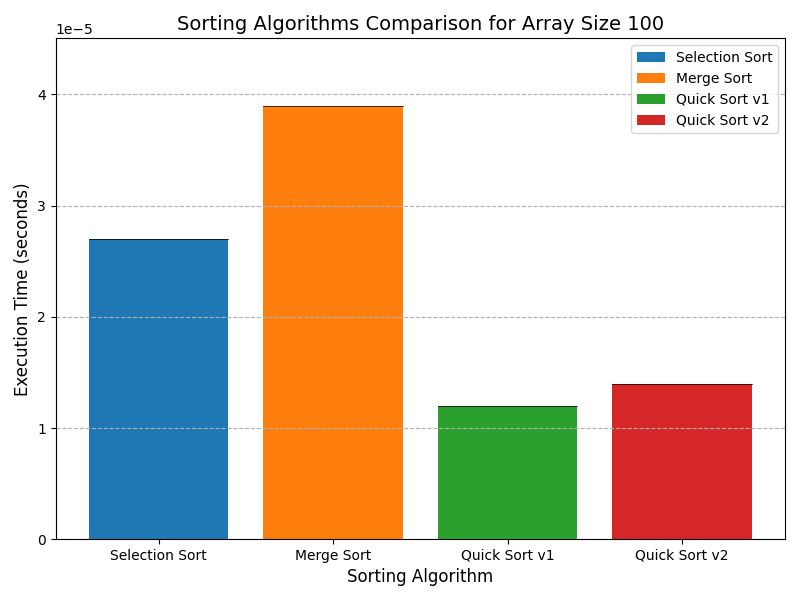
\includegraphics[width=0.5\textwidth]{"../img/b_Figure_5.png"}
    \caption{Comparison of Selection Sort, Merge Sort, and the two versions of Quick Sort when sorting an array of size 1000.}
    \label{fig:image5}
\end{figure}

\begin{figure}[htbp]
    \centering
    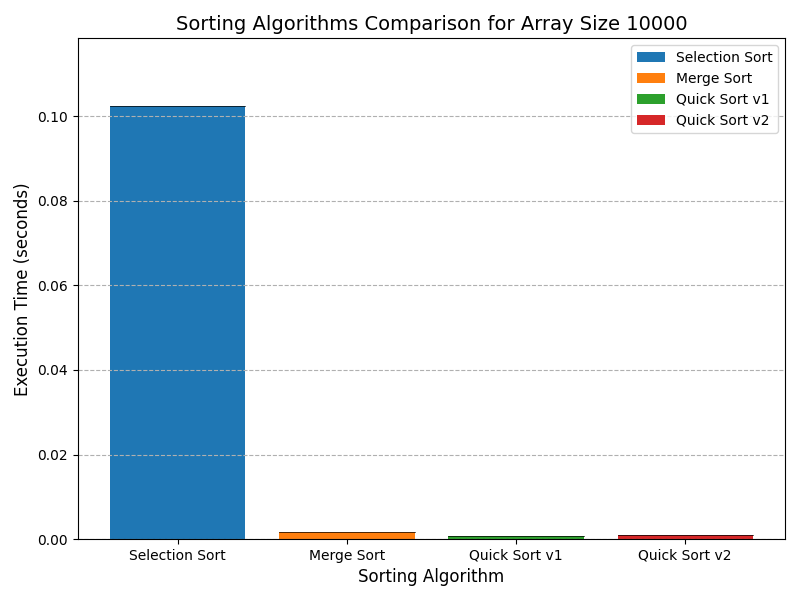
\includegraphics[width=0.5\textwidth]{"../img/b_Figure_6.png"}
    \caption{Comparison of Selection Sort, Merge Sort, and the two versions of Quick Sort when sorting an array of size 10000.}
    \label{fig:image6}
\end{figure}

\begin{figure}[htbp]
    \centering
    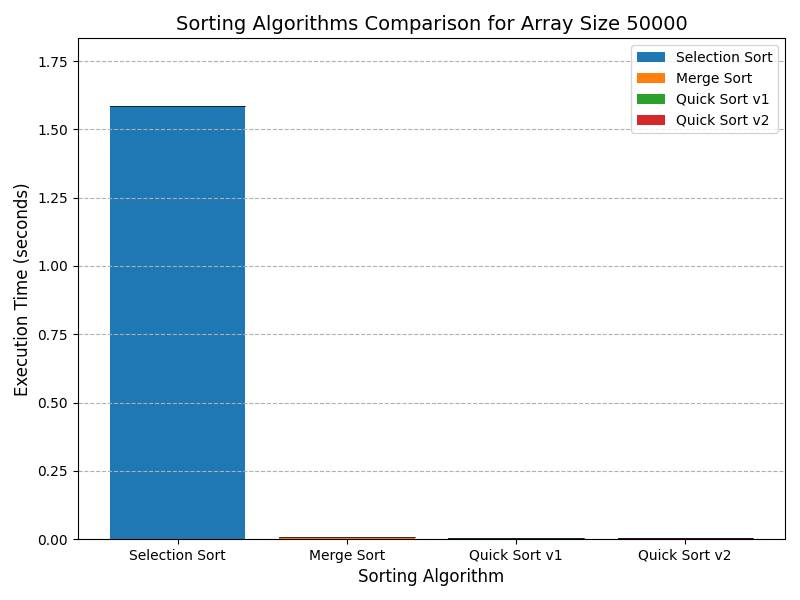
\includegraphics[width=0.5\textwidth]{"../img/b_Figure_7.png"}
    \caption{Comparison of Selection Sort, Merge Sort, and the two versions of Quick Sort when sorting an array of size 50000.}
    \label{fig:image7}
\end{figure}

\begin{figure}[htbp]
    \centering
    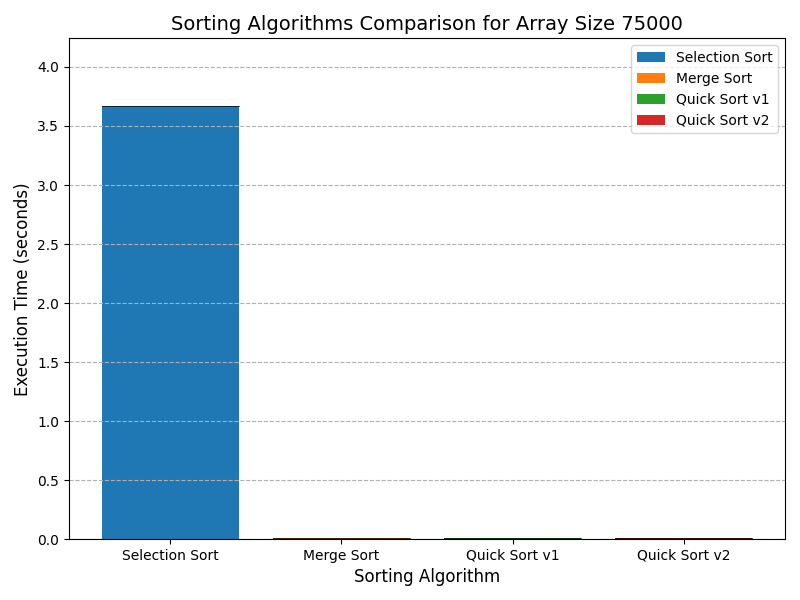
\includegraphics[width=0.5\textwidth]{"../img/b_Figure_8.png"}
    \caption{Comparison of Selection Sort, Merge Sort, and the two versions of Quick Sort when sorting an array of size 75000.}
    \label{fig:image8}
\end{figure}

\begin{figure}[htbp]
    \centering
    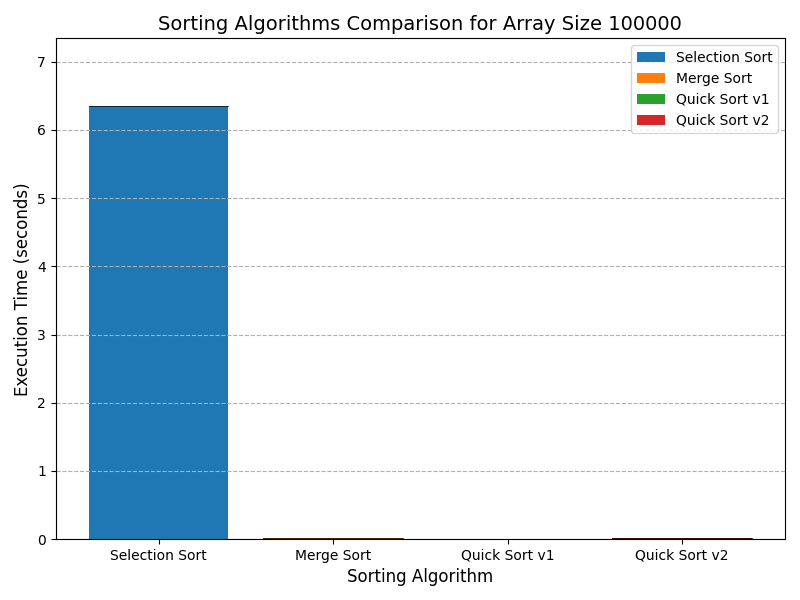
\includegraphics[width=0.5\textwidth]{"../img/b_Figure_9.png"}
    \caption{Comparison of Selection Sort, Merge Sort, and the two versions of Quick Sort when sorting an array of size 100000.}
    \label{fig:image9}
\end{figure}

\begin{figure}[htbp]
    \centering
    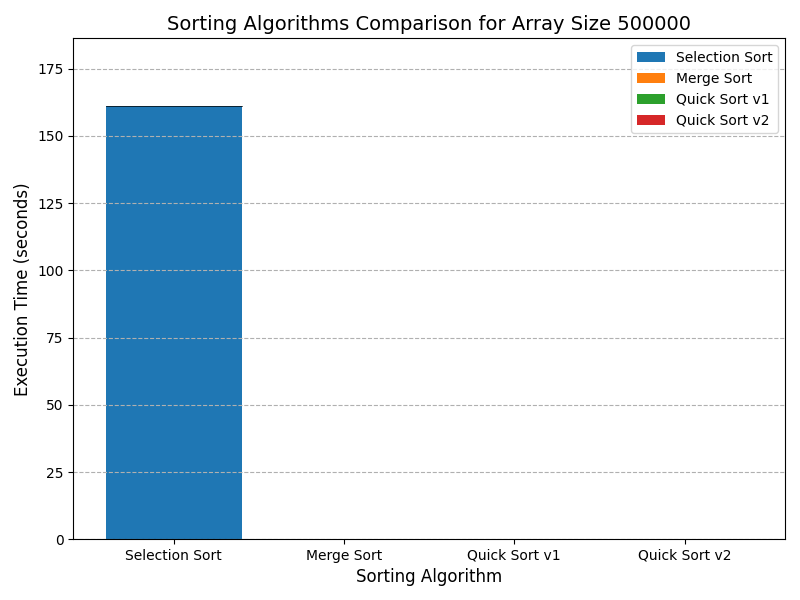
\includegraphics[width=0.5\textwidth]{"../img/b_Figure_10.png"}
    \caption{Comparison of Selection Sort, Merge Sort, and the two versions of Quick Sort when sorting an array of size 500000.}
    \label{fig:image10}
\end{figure}

\clearpage

The graphs above compare the efficiency of sorting algorithms when the input array size is fixed. In Figure \ref{fig:image5}, the graph shows that Selection Sort is the least efficient algorithm. This is because Selection Sort has a time complexity of $O(n^2)$.

\par\medskip 

The graph also shows that the two versions of Quick Sort are the most efficient algorithms. This is because Quick Sort has a time complexity of $O(n \log n)$. Additionally, the graph demonstrates that the second version of Quick Sort is more efficient than the first version. The higher constant factor in the second version, due to the pivot swap with the last element of the array, makes the first version more efficient. 

\par\medskip

The graph further illustrates that Merge Sort is more efficient than Selection Sort, but less efficient than the two versions of Quick Sort. This is because Merge Sort has a time complexity of $O(n \log n)$, which is more efficient than Selection Sort, but less efficient than Quick Sort.

\end{document}
